\begin{frame}
  \frametitle{Perfused Muscle Tissue: Heart, Kidneys}
  \begin{itemize}
  \item \emph{solid--fluid mixture}, large content of water, but almost solid
    \dots
  \item transport in soft tissue
    \begin{itemize}
    \item nutrient supply / drainage of waste
    \item transport of oxygen
    \item transport of ions  
    \end{itemize}
  \item coupling = feedback
    \begin{itemize}
    \item perfusion $\rightarrow$ muscular activity, contraction
      $\rightarrow$ perfusion
    \end{itemize}
  \end{itemize}
  \begin{center}
    \begin{minipage}{0.28\linewidth}
      \scriptsize
      multiple channel systems \\
      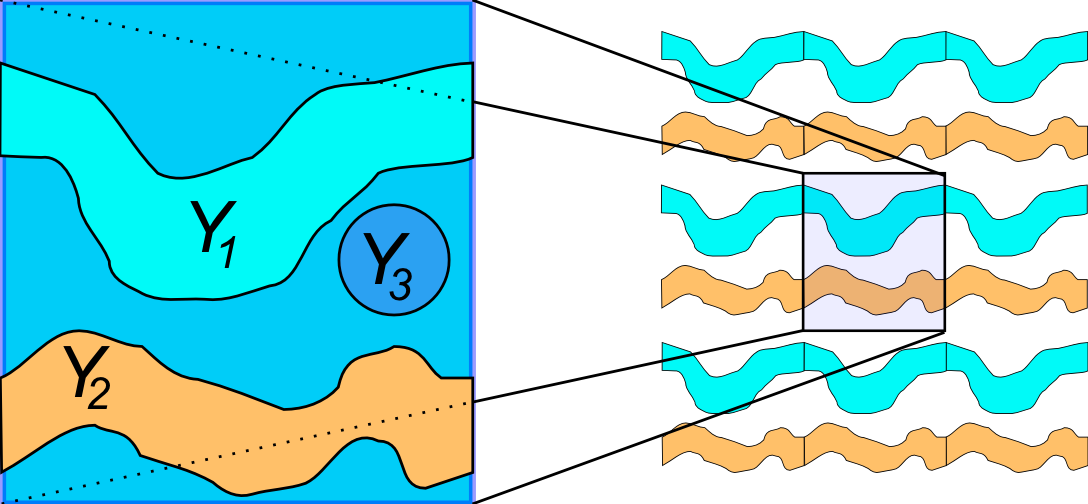
\includegraphics[width=0.9\linewidth]
      {\figDirMacroPerfusion/fig_2porous_Y-domain_new} \\

      \red{heart}: \\ $p_1$ arterial, $p_2$ venous pressure
      $p_v$ ventricular pressure traction

      \blue{kidneys}: \\ $p_1$ arterial, $p_2$ venous, $p_3$ filtrate pressure
      $p_{\rm abd}$ abdominal pressure traction
    \end{minipage}
    \hfill
    \begin{minipage}{0.35\linewidth}
      \scriptsize
      application: heart \\
      \centering
      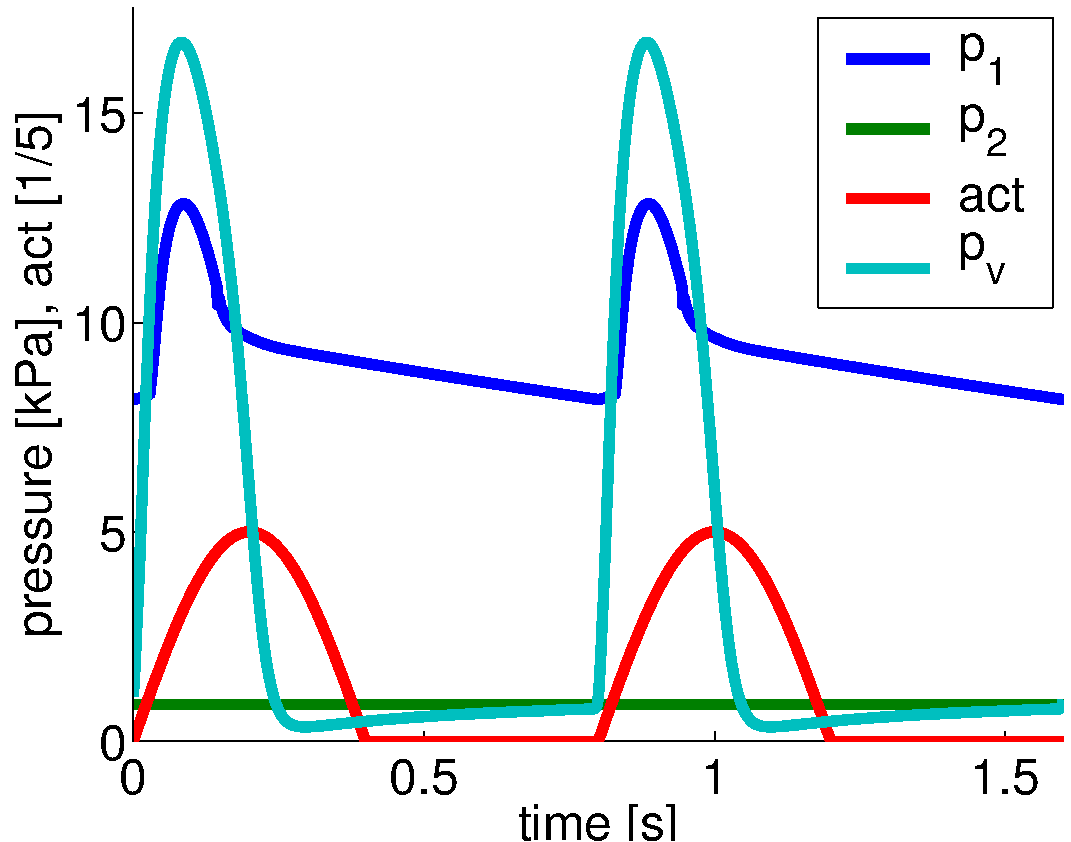
\includegraphics[width=0.6\linewidth]
      {\figDirMacroPerfusion/loads_heart} \\
      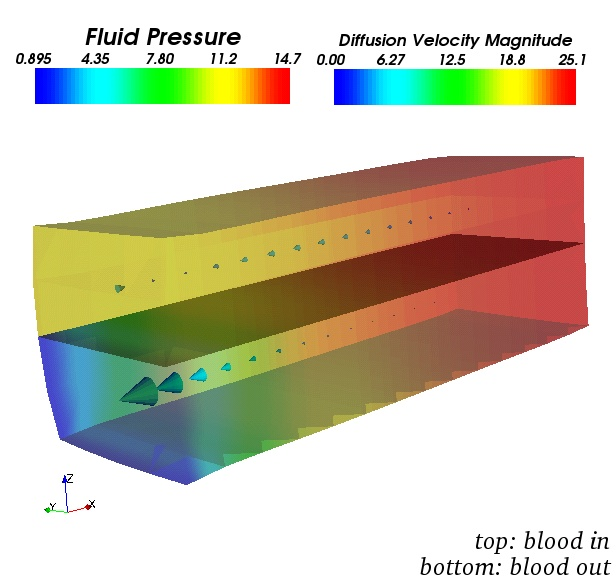
\includegraphics[width=0.6\linewidth]
      {\figDirMacroPerfusion/perfusion_heart_block_4_0026}
    \end{minipage}
    \hfill
    \begin{minipage}{0.35\linewidth}
      \scriptsize
      application: kidneys \\
      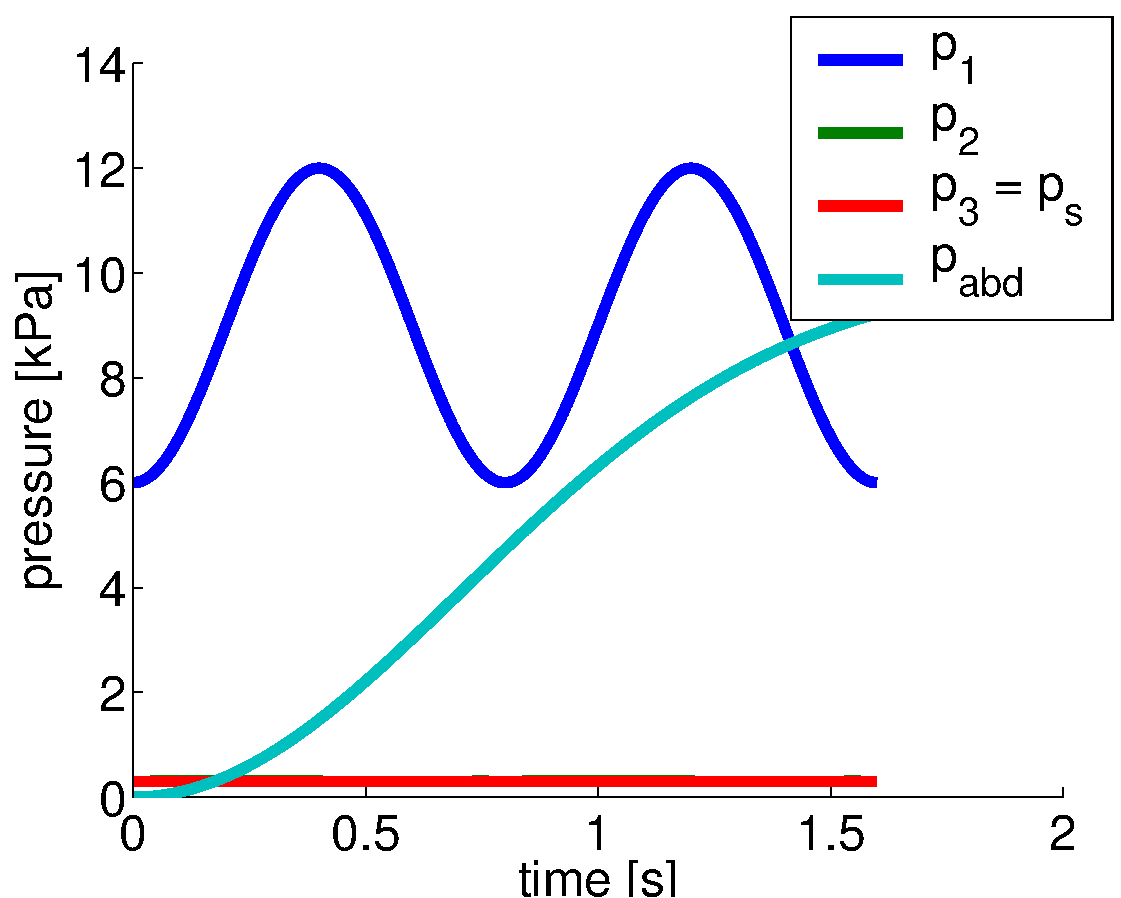
\includegraphics[width=0.6\linewidth]
      {\figDirMacroPerfusion/loads_kidney} \\
      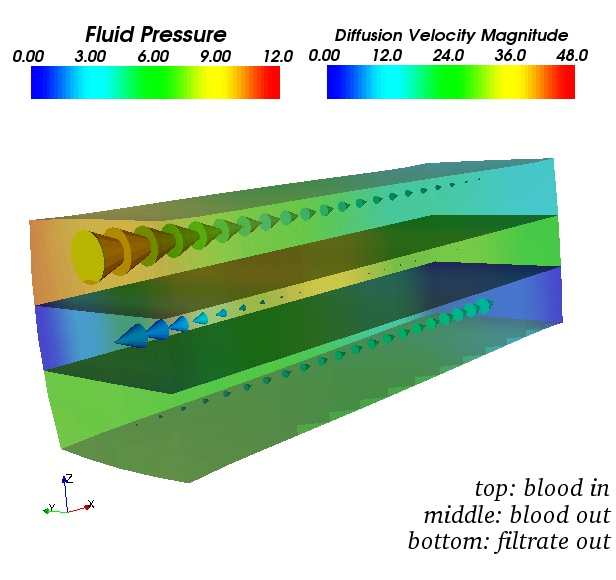
\includegraphics[width=0.6\linewidth]
      {\figDirMacroPerfusion/perfusion_kidney_block_3_0055}
    \end{minipage}
  \end{center}
\end{frame}
